% ===============================
%        Corrector Response
% ===============================
\section{\review{Response of correctors}}
\label{section:decapoles:chromaticity}

As seen in \cref{fig:introduction:lhc_arc_cell}, the LHC is equipped with decapole correctors. Those
magnets are part of the LHC's design report, aiming at correcting the field errors of the main
dipoles. Those correctors, denominated \textit{MCD}, are specific to each beam and are placed after
every second dipole, totaling 1232 in number~\cite{venturini_delsolaro_magnetic_2005}.  MCDs are
nested with octupolar correctors, \textit{MCO}. The pair of those correctors of often referred to as
\textit{MCDO}. 
It is not possible to individually power each corrector. Rather, a circuit consists of a whole arc.
There are in total 16 circuits to control the correctors of both beams and 8 arcs.
\Cref{fig:decapoles:decapole_picture} shows a picture taken of decapoles on a test bench.

\begin{figure}
    \centering
    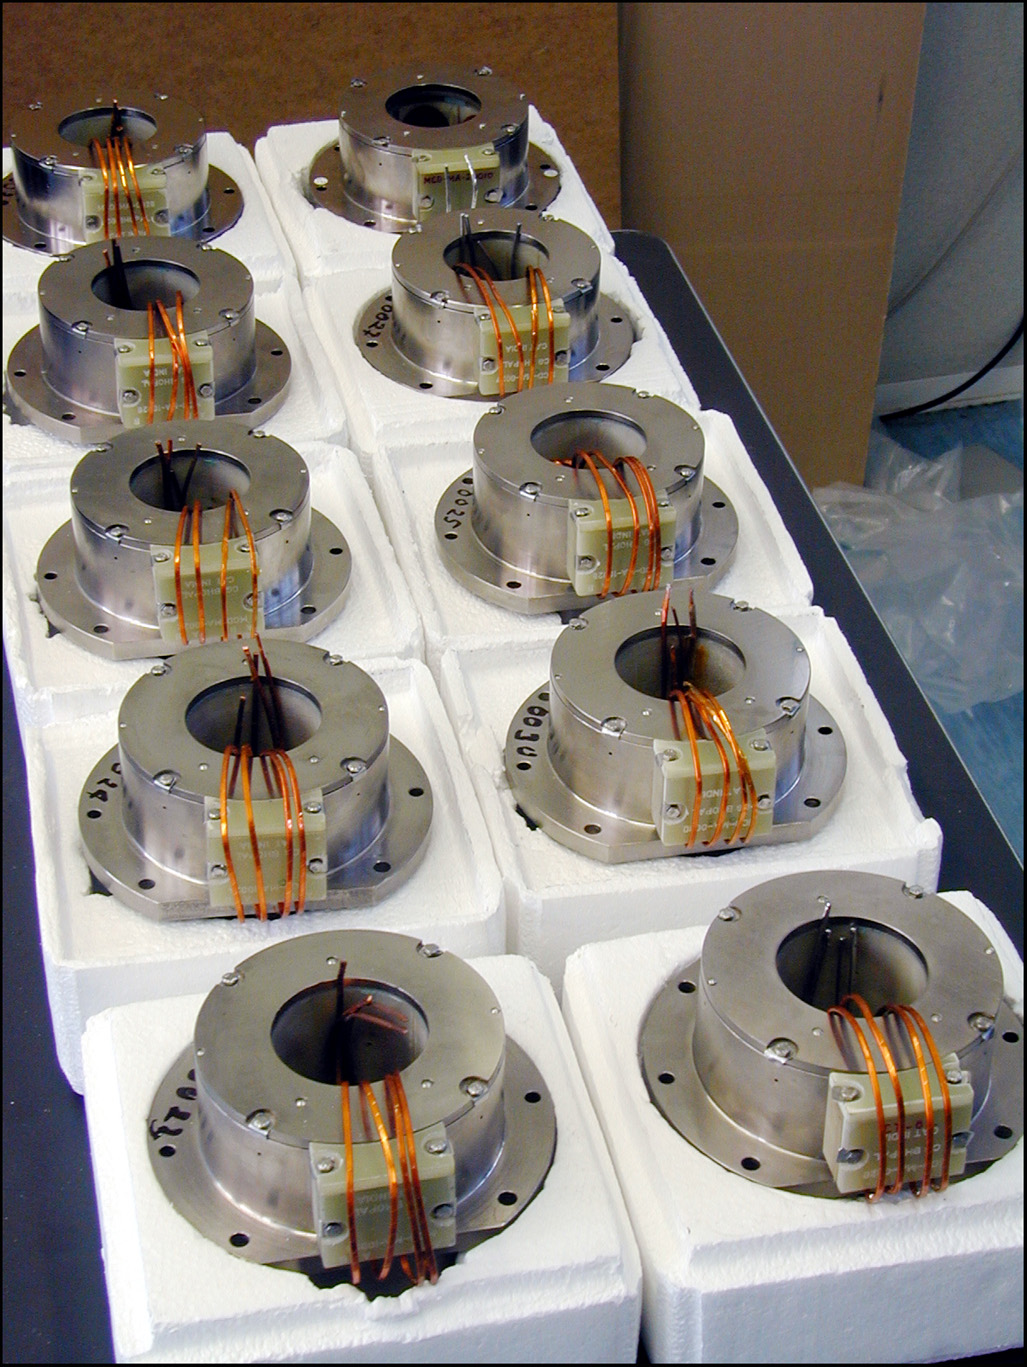
\includegraphics[width=0.4\textwidth]{./images/decapoles_real_pic.jpg}
    \caption{Decapoles on a test bench, being inspected after
    manufacturing~\cite{noauthor_ten_2001}.}
    \label{fig:decapoles:decapole_picture}
\end{figure}

The important characteristics of the magnetic fields of correctors are their main field transfer
function (or \textit{response}), the field quality and possible crosstalk, as MCOs and MCDs are
nested~\cite{venturini_delsolaro_magnetic_2005}. To resolve the previously stated discrepancy, it is
essential to investigate the decapole correctors themselves, to rule them out as the source of this
difference.

%% -------- Strengths at Injection
%\paragraph{Strengths at Injection}
%
%%\begin{wraptable}{r}{0.4\textwidth}
%\begin{table}
%    \centering
%    \begin{tabular}{lr}
%        \toprule
%        Circuit   & $K_5 [\textrm{m}^{-5}]$ \\
%        \midrule
%        Beam 1    & \\
%        \hspace{2mm}RCD.A12B1 & $-4582$ \\
%        \hspace{2mm}RCD.A23B1 & $-5106$ \\
%        \hspace{2mm}RCD.A34B1 & $-4855$ \\
%        \hspace{2mm}RCD.A45B1 & $-4577$ \\
%        \hspace{2mm}RCD.A56B1 & $-4125$ \\
%        \hspace{2mm}RCD.A67B1 & $-5166$ \\
%        \hspace{2mm}RCD.A78B1 & $-6827$ \\
%        \hspace{2mm}RCD.A81B1 & $-5500$ \\
%        Beam 2    & \\
%        \hspace{2mm}RCD.A12B2 & $-4490$ \\
%        \hspace{2mm}RCD.A23B2 & $-5155$ \\
%        \hspace{2mm}RCD.A34B2 & $-4825$ \\
%        \hspace{2mm}RCD.A45B2 & $-4619$ \\
%        \hspace{2mm}RCD.A56B2 & $-4064$ \\
%        \hspace{2mm}RCD.A67B2 & $-5066$ \\
%        \hspace{2mm}RCD.A78B2 & $-6866$ \\
%        \hspace{2mm}RCD.A81B2 & $-5446$ \\
%        \bottomrule
%    \end{tabular}
%    \caption{Strength of decapolar correctors at injection energy for FiDeL corrections.}
%    \label{tab:decapoles:strength_rcd_fidel}
%%\end{wraptable}
%\end{table}
%
%At injection energy, the decapolar correctors are powered to a static strength. New optics introduced
%throughout the years often have for effect to vary slightly the $\beta$-function along the ring,
%having thus an impact on the chromaticity, as seen in
%\cref{eq:detuning_effects:chromaticity_strength}. New corrections are then computed via FiDeL to
%account for it.
%Although those corrections vary throughout the years, the shift is in practice fairly negligible.
%\Cref{tab:decapoles:rdts:correction_f1004_k5}, a bit further in this chapter, shows the strength of
%the correctors and the related circuits at injection energy for the optics deployed in 2024.


The full third term of the chromaticity function is highlighted in
\cref{eq:decapoles:chromaticity_highlight}. Details on chromaticity are given
in \cref{subsection:concepts:chromaticity}.

\begin{equation} 
    Q (\delta) = Q_0 + Q' \delta + \frac{1}{2!} Q'' \delta^2 
                     + \colorbox{yellow!50}{$\displaystyle  \frac{1}{3!}  Q''' \delta^3$}
                     + \mathcal{O}(\delta^4).
    \label{eq:decapoles:chromaticity_highlight}
\end{equation}

This third order, generated by leading order by decapoles in a region of non-zero linear dispersion,
is related to the $\beta$-function, the dispersion and the normalized strength $K_5 [\text{m}^{-5}]$
of the decapolar correctors:

\begin{equation}
    \begin{aligned}
        \Delta Q_x''' &=  &\frac{1}{4\pi} K_{5} L \beta_x D_x^{3}\\
        \Delta Q_y''' &= -&\frac{1}{4\pi} K_{5} L \beta_x D_x^{3}.
    \end{aligned}
\end{equation}

During Run~3's commissioning, the routine measurement and correction of $Q''$ and $Q'''$ have been
established. These corrections provide a valuable opportunity to analyze the response of the
decapole correctors, \textit{MCDs}. By studying this response, it is possible to determine whether
the source of the $Q'''$ discrepancy originates from a miscalibration of the decapolar
correctors or not.
\Cref{figure:decapoles:chromaticity:dq3_comparison} shows the chromaticity function measured during
Run~3's commissioning in 2022 with the nominal FiDeL corrections and with further beam-based 
corrections computed analytically and applied on top.

\begin{figure}[!htb]
    \centering
    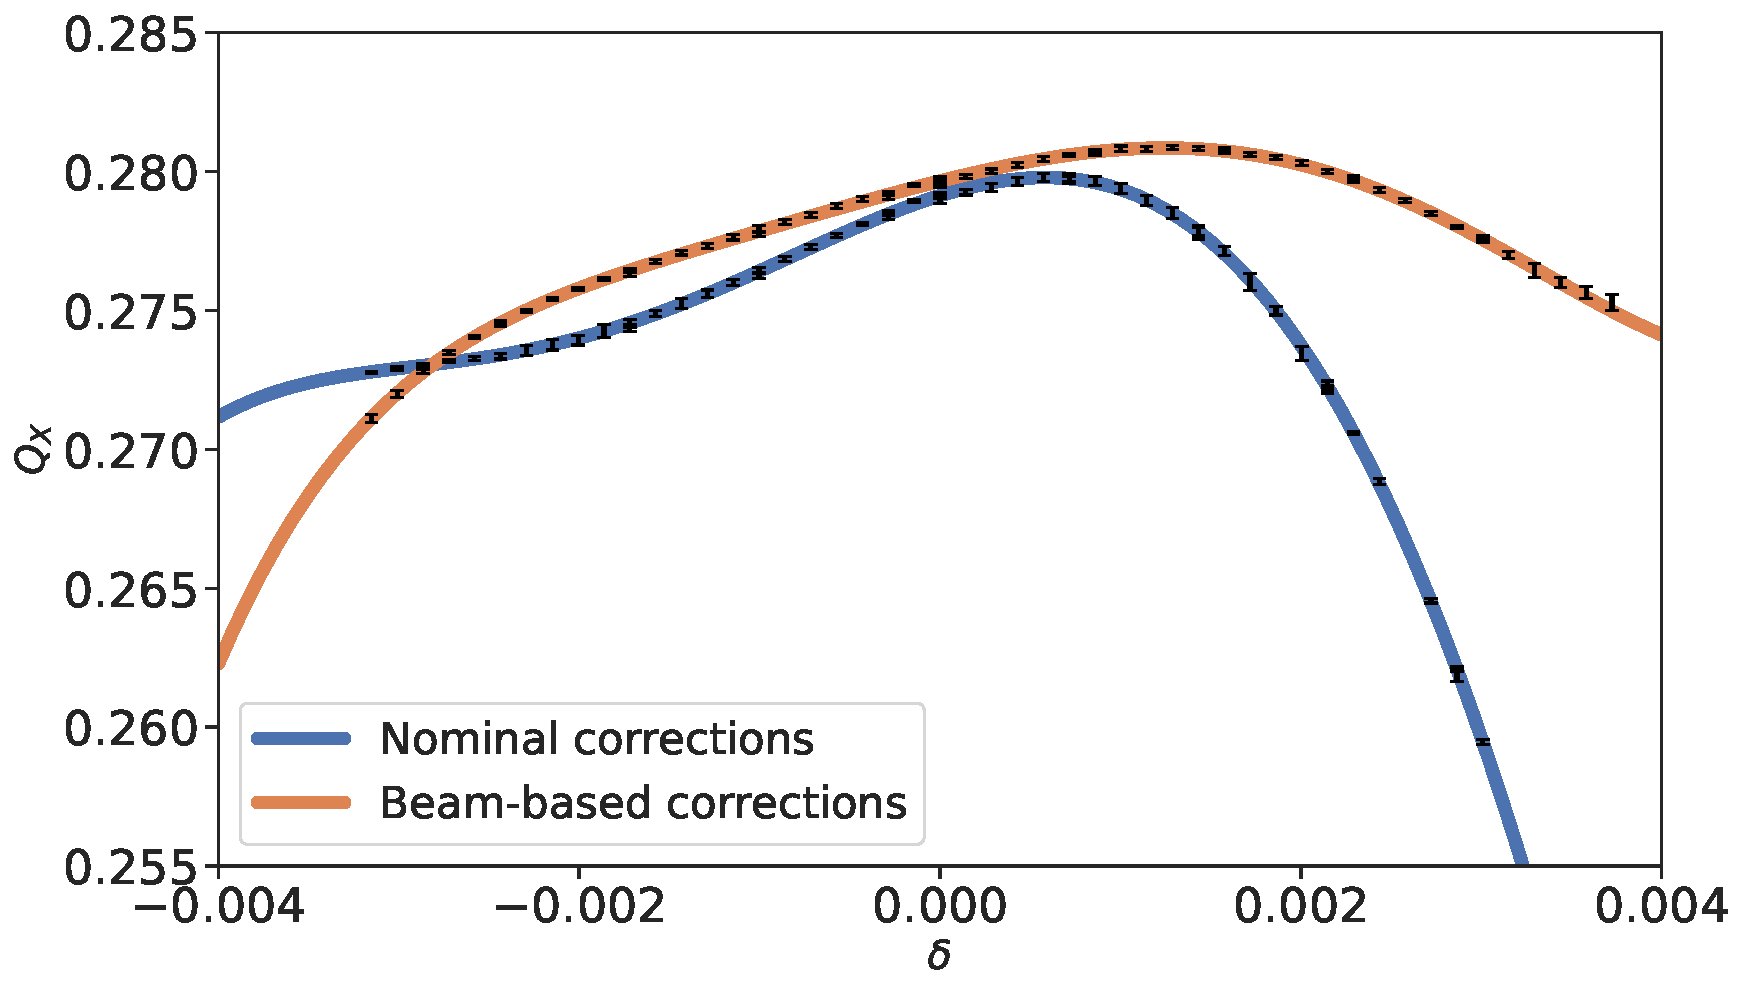
\includegraphics[width=0.8\columnwidth]{images/nominal_vs_beam_based_corrections.pdf}
    \caption{Chromaticity of the horizontal plane of Beam 1 during Run 3's commissioning, with
    nominal corrections based on the magnetic model and beam-based corrections aimed at correcting
     $Q''$ and $Q'''$.}
    \label{figure:decapoles:chromaticity:dq3_comparison}
\end{figure}

The nominal and corrected $Q'''$ values are shown in
\cref{table:decapoles:chromaticity:dq3_before_after_beam_based}, with the shift in $Q'''$ for each
beam and axis. A good agreement between the measurements and simulations can be seen.

\begin{table}[!htb]
    \centering
    \begin{minipage}{0.45\linewidth}
        \centering
        \begin{tabular}{lrr}
          \toprule
                  &  \multicolumn{2}{c}{$Q''' [10^6]$}  \\
            Plane & Nominal & Beam-Based \\
          \midrule
            Beam 1    &   & \\
            \hspace{2mm}X     &  -3.36 ± 0.04 &  -1.02 ± 0.03 \\
            \hspace{2mm}Y     &   1.62 ± 0.05 &   0.12 ± 0.02 \\
            Beam 2    &           &               \\
            \hspace{2mm}X     &  -2.72 ± 0.08 &  -0.64 ± 0.03 \\
            \hspace{2mm}Y     &   1.54 ± 0.06 &   0.14 ± 0.03 \\
            \bottomrule
        \end{tabular}
    \end{minipage}%
    \hspace{1cm} % Adjust horizontal space between tables
    \begin{minipage}{0.45\linewidth}
        \centering
        \begin{tabular}{rr}
          \toprule
          \multicolumn{2}{c}{$\Delta Q''' [10^6]$}\\
          Meas.   & Simulation \\
          \midrule
          & \\
          2.3 ± 0.1 &   2.5 \\
          -1.5 ± 0.1 &  -1.4 \\
          &  \\
          2.1 ± 0.1  &  2.5\\
          -1.4 ± 0.1 & -1.4\\
          \bottomrule
        \end{tabular}
    \end{minipage}
    \caption{Third order chromaticity obtained during Run~3 commissioning, with nominal and
             beam-based corrections aimed at correcting $Q''$ and $Q'''$. Response of the correctors
             between the two configurations is also given for both measurement and simulation.}
    \label{table:decapoles:chromaticity:dq3_before_after_beam_based}
\end{table}
  

The agreement between simulations and measurements confirms that the decapole correctors are
functioning as intended. No errors in their calibration or response function (current to strength)
have been identified that could explain the observed $Q'''$ discrepancy.
%No noticeable cross-talk between magnets or hysteresis have been identified.


% ===============================
%        Bare Chromaticity
% ===============================
\section{\review{Bare Chromaticity}}
% 2022-10-19

Complementary to the measurements of $Q'''$ shifts with varying decapolar strengths, measurements of
the bare machine, without any correctors powered, can provide valuable insights. These measurements
help rule out potential crosstalk between the octupolar and decapolar correctors, which are
physically nested, and allow for a clearer understanding of the contribution of octupolar correctors
to $Q'''$. Additionally, they offer a direct and clean comparison to the magnetic model. The
obtained results are presented in \cref{fig:decapoles:bare_chromaticity}.

\begin{figure}[!htb]
    \begin{subfigure}{0.49\textwidth}
        \centering
        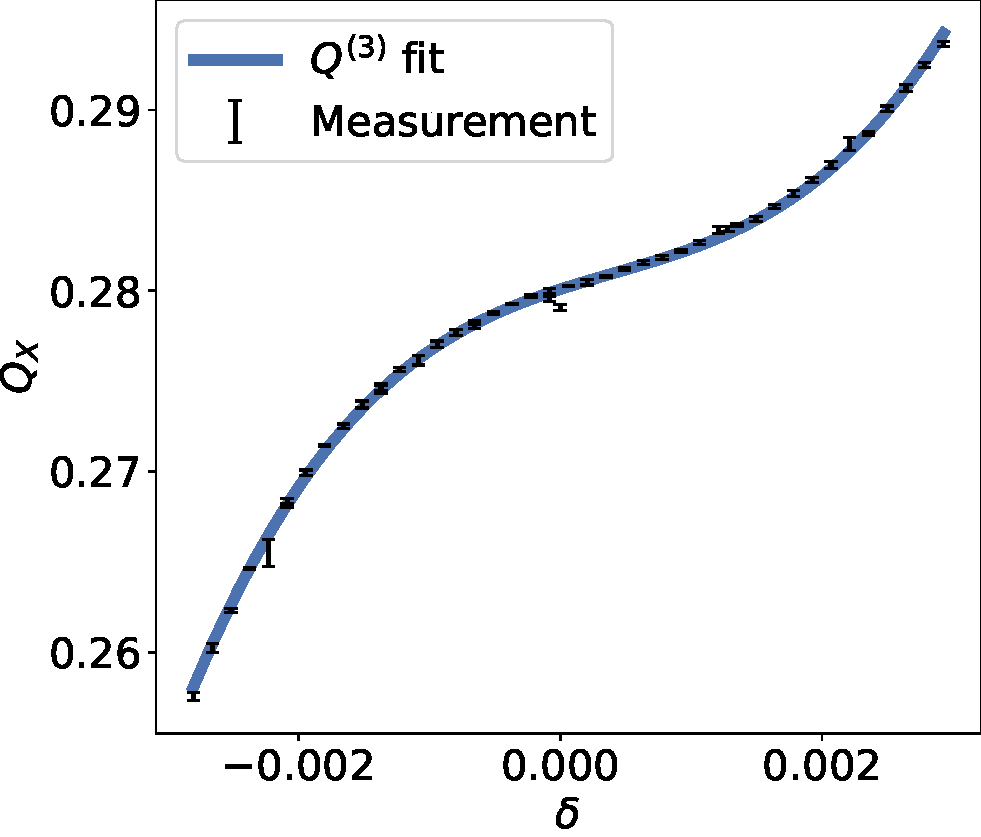
\includegraphics[width=\textwidth]{./images/bare_chromaticity/Beam1_Qx.pdf}
        \caption{$Q_x$ Beam 1}
    \end{subfigure}
    \hfill
    \begin{subfigure}{0.49\textwidth}
        \centering
        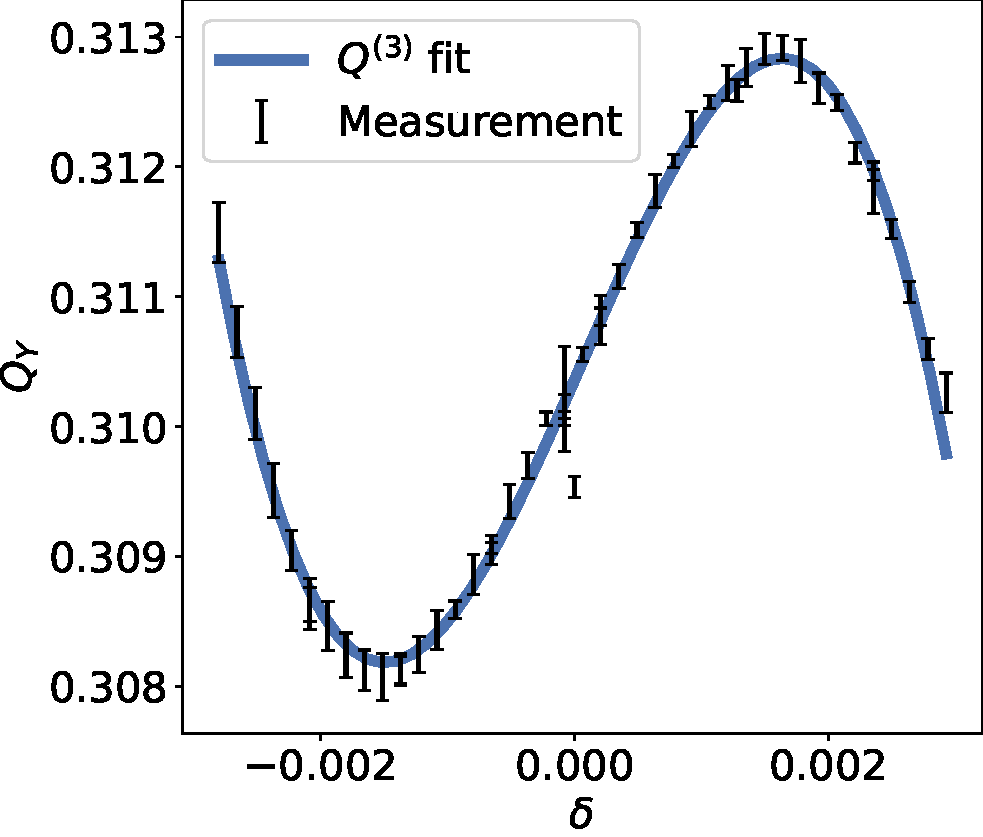
\includegraphics[width=\textwidth]{./images/bare_chromaticity/Beam1_Qy.pdf}
        \caption{$Q_y$ Beam 1}
    \end{subfigure}
    %
    \\
    %
    \begin{subfigure}{0.49\textwidth}
        \centering
        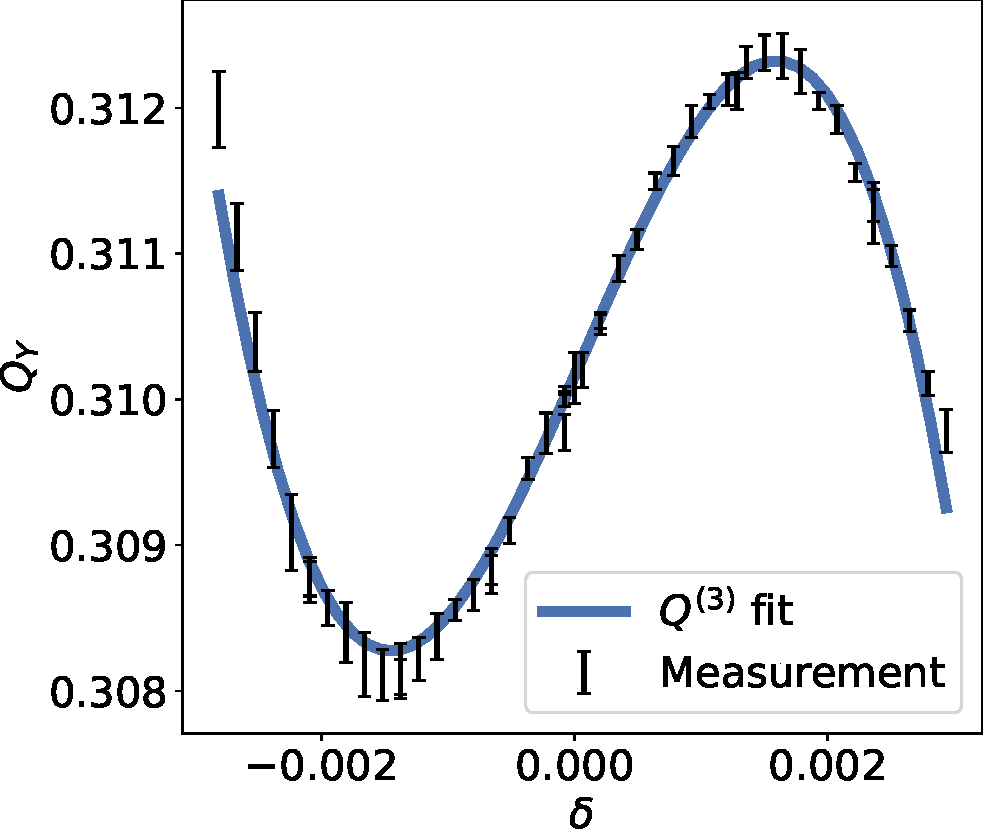
\includegraphics[width=\textwidth]{./images/bare_chromaticity/Beam2_Qy.pdf}
        \caption{$Q_x$ Beam 2}
    \end{subfigure}
    \hfill
    \begin{subfigure}{0.49\textwidth}
        \centering
        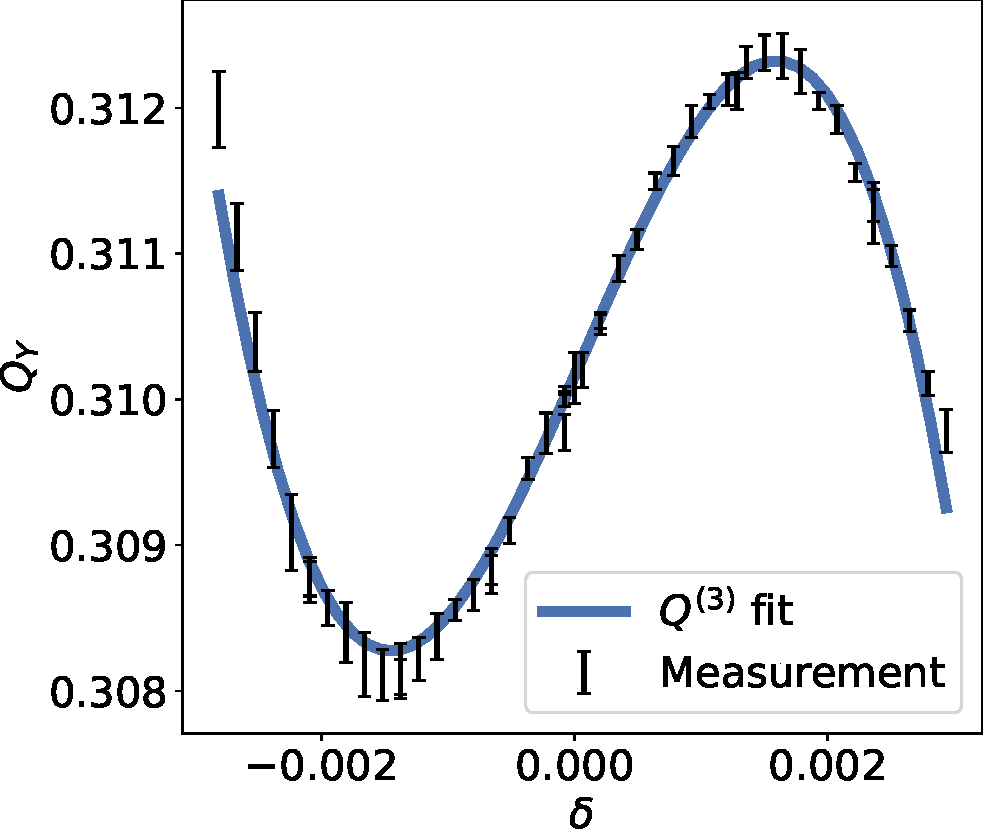
\includegraphics[width=\textwidth]{./images/bare_chromaticity/Beam2_Qy.pdf}
        \caption{$Q_y$ Beam 2}
    \end{subfigure}
    \caption{Fit of the chromaticity function for the chromaticity measurement performed with 
    octupole and decapole correctors powered off. The fit includes all orders up to third.}
    \label{fig:decapoles:bare_chromaticity}
\end{figure}

Simulations have been run with MAD-X and PTC including fields errors from normal sextupole to 
decahexapole. The expected $Q'''$ values are presented
in~\cref{table:decapoles:bare_chromaticity:virgin_dq3} and compared to the measured ones along with
the ratio between the two.

\begin{table}[tbh]
    \centering
    \begin{tabular}{rrrc}
    \hline
        \toprule
        Quantity  &  Measured $[10^6]$        &  Simulated $[10^{6}]$          &   Ratio       \\
        \midrule
        \multicolumn{1}{l}{Beam 1}    &                           &                                &               \\
         $Q'''_x$ &     $ 2.95 \pm 0.04$      &       $ 6.94 \pm 0.02$         &  $0.43 \pm 0.01$\\
         $Q'''_y$ &     $-1.82 \pm 0.04$      &       $-4.29 \pm 0.01$         &  $0.42 \pm 0.01$\\
        \multicolumn{1}{l}{Beam 2}    &                           &                                &               \\
         $Q'''_x$ &     $ 3.06 \pm 0.07$      &       $ 7.03 \pm 0.02$         &  $0.44 \pm 0.01$\\
         $Q'''_y$ &     $-1.72 \pm 0.02$      &       $-4.27 \pm 0.01$         &  $0.42 \pm 0.01$\\
         \bottomrule
    \end{tabular}
    \caption{Measured and simulated third order chromaticity with octupole and decapole correctors
    turned off. The simulations include field errors from sextupoles to decahexapole (normal
    sextupole to decahexapole).}
    \label{table:decapoles:bare_chromaticity:virgin_dq3}
\end{table}

The observed discrepancy between the measurements and simulations persists both with the FiDel 
corrections applied and with the correctors turned off. Similarly, measuring significantly different 
lower-order chromaticities and working points, the discrepancy remains consistently around a factor 
of $2$ between the measured and expected $Q'''$. This suggests that the source of the discrepancy lies 
elsewhere. One possible explanation could be an error in the systematic decapolar component of the 
main dipoles in the magnetic model. However, relying solely on $Q'''$ does not allow for a definitive 
conclusion, as higher-order effects like non-linear dispersion or non-linear momentum compaction
factor could also contribute. To resolve this, additional observables, such as chromatic amplitude
detuning, will be required for further investigation.


\FloatBarrier